\documentclass{article}
\usepackage{natbib}
\usepackage{graphicx}
\usepackage{float}

\title{High-Performance Data Analysis on Janus using Apache Spark}
\author{Nick Vanderweit \\
        Ning Gao \\
        Anitha Ganesha \\
        Michael Kasper}

\begin{document}
\maketitle

\section{Introduction}
Over the past decade, there has been considerable interest in high-level
strategies for evaluating algorithms in parallel over large data sets.
Google's seminal MapReduce paper \citep{dean-mapreduce} describes such a
general strategy, which had already been in use at Google at the time of
publication, for building highly-scalable parallel applications out of small
serial functions. In general, phrasing data parallelism in terms of
higher-order functions on parallel data structures has proven fruitful
for many applications. In this paper, we evaluate Spark, a library
designed to address some of the shortcomings of MapReduce, on an existing
supercomputer.

In the MapReduce model, data is broken into \emph{splits} of a given size
before processing. These are stored on a distributed filesystem as key/value
pairs. The master node then distributes splits among the remaining workers.
Each of these workers runs a \emph{Map} on its split, computing for each
key/value pair $(k_1, v_1)$ another pair $(k_2, v_2)$. Each of these output
pairs is stored on the filesystem and the master is informed of their
locations. The master node proceeds by forwarding these intermediate pairs to the
\emph{Reduce} workers, which are responsible for combining the results for each
intermediate key.

A commonly-used example for this process is a distributed word count. First,
the input file (e.g. a large database dump containing posts on an Internet
forum) is broken into splits of a given size (say 64MB). The splits store
$(k, v)$ pairs such that each $v$ is a record (a post). The \emph{Map} task
is responsible for mapping each record to a set of (word, count) pairs,
which are written to the filesystem.

The next step is for a \emph{Reduce} worker to sort these records by key
and then sum together the values for each given key, and write out
a set of (word, count) records where the keys are now unique.

This simple example has interesting implications for MapReduce in general.
We can see that \emph{Map} tasks are highly-parallel, but \emph{Reduce}
introduces a serial bottleneck. In cases like parallel word count, where the
\emph{Reduce} is associative and commutative (i.e. forms a commutative
semigroup over the set of values), there is an additional opportunity for
parallelism. As such, MapReduce provides an additional task, called a
\emph{Combiner}, which assumes this structure and can be used to distill
the intermediate $(k, v)$ pairs before a \emph{Reduce}.

We can also see from this example a significant limitation of MapReduce: each
intermediate $(k, v)$ set is written to the distributed filesystem.  As such,
in order for MapReduce to be efficient, the individual tasks must be very
large.

However, some algorithms are not well-described by a simple map-and-then-reduce
pattern, and require multiple iterations.  If each iteration is small, the
algorithm's performance will be bottlenecked by this file I/O. For these
problems, another approach is needed.

Spark was designed at the UC Berkeley AMPLab to address these concerns using a
more flexible abstraction for distributed data \citep{zaharia}. Rather than
assuming that all intermediate data is stored on a filesystem, Spark uses
\emph{Resilient Distributed Datasets}, or RDDs, to represent data that is
stored on disk, cached in memory, or possibly has not been computed yet at all
\citep{zaharia_rdd}.  It is primarily targeted toward Scala, a statically-typed
functional language for the Java Virtual Machine.

\section{Overview}

\section{Evaluation}
% janus
    % overview
    % describe what spark test where
    % installed and tested on janus
    % janus specs
    % spark, scala version
    % test to determine performance
    % reason for spark (diskless)
    % installation (default???)
    % version number (Spark 0.8.0, Scala 2.9.3)
    % find ideal configurations

        % we conducted our evaluaion of Spark
        % on University of Colorado's Janus super computer
        % Janus consists of 1,368 nodes, each contains
        % two size core Intel Xeon Westmere-EP chips at 2.8 GHz
        % total of 12 cores per node
        % Each core has 2 GB of 1333 MHZ DDR Ram
        % 24 GB per node (REF)

        % our project used Spark version 0.8.0
        % along with Scala 2.9.3
        % accessed files both from Janus's Lustre and ???
        % aim to assess spark performance on janus
        % determine optimal configurations

\subsection{Testing}
% grep
    % overview
        % used example from googles first paper (ref)
        % searching for a pattern in large text file
        % return line count with matches
    % files sizes
        % two different tests, 20GB, 100GB
        % memory limitation of 1 node 24 gb
    % node core counts
        % small test ranged from 1 - 5 nodes
        % large test ranged from 5 - 50 nodes
        % 10 trials were performed on each config
        % each test utilized all 12 cores
    % serial runtime
        % the spark parallel time was compared to serial
        % serial time was unix grep command
    % workers per node
        % other configuration setting was workers per node
        % what is worker? (ref)
        % compared on small test

        % following exampe of googles first paper on MapReduce
        % first test performed a parallel grep over large text file
        % returning line count of found results
        % two different tests, different files sizes
        % required to fit entire file in memory
        % first test, over 1-5 nodes on 20GB file
        % second test, over 5-50 nodes on 100GB file
        % each trials utilzed all 12 cores of each node
        % 10 trials were performed with each configuration
        % to compute average runtimes
        % to compute speedup, the unix grep runtime was used a serial
        % finally, during first test over 20GB file
        % played with number of workers per core
        % workers execute application on their portion of distrubted data set

% page rank
    % overview
    % ...

\subsection{Results}
% cores grep test
    % scale up, workers per node (graph)
    % runtimes of several combinations of workers per node
    % runtimes compare with the serial runtime of 20gb file of 1120s
    % perhaps 2-3 workers has a slight performance increase over 1 worker
    % clear that 6 and 12 workers are not ideal
    % additional overhead being the problem

        % first testing obverve scaling on 20GB grep task
        % also play with workers per node
        % see scales and ideal config
        % figRef shows rutimes grep 20GB file from 1-5, 12-60 processes
        % comparing to the unix grep serial runtime of 1,120 seconds
        % each line represents a different config of workers per core
        % clearly see that 6 and 12 were significanlty slower
        % most likely due to additional communication overhead
        % while 1-3 workers relatively similar runtimes
        % maybe be a slight performance increase using 2-3 workers per node

    \begin{figure}[H]
        \centering
        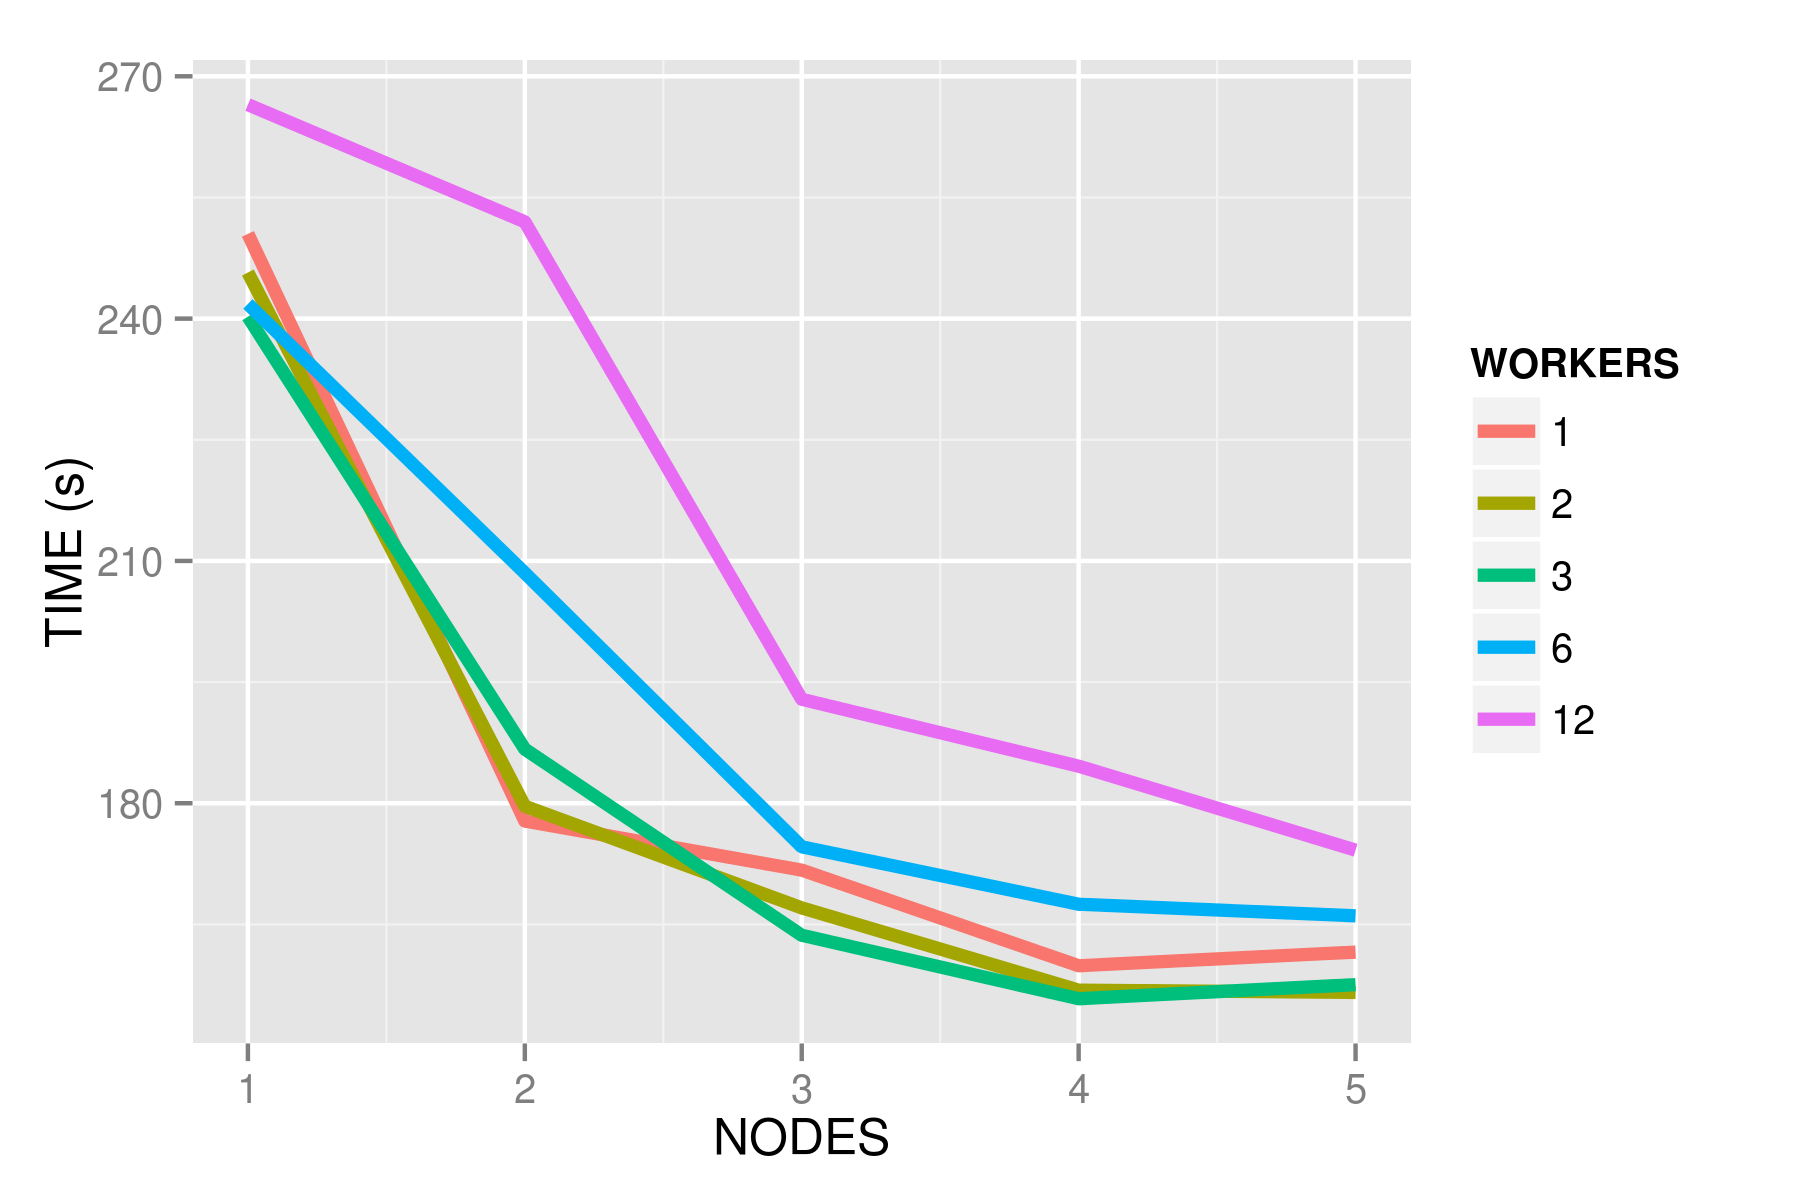
\includegraphics[width=90mm]{images/workerPerNodeTimes.png}
        \caption{Grep runtimes with different workers per node over 20GB file}
        \label{fig:workNodeTime}
    \end{figure}

    % speedup representation (ref)
    % starts with 12 cores, fare less than linear speedup
    % begins to level out around 4 nodes
    % 1-3 workers actually starts to decrease

        % imageRef illustrates this test in terms of speedup
        % as one nodes consists of 12 cores
        % the initial speedup shown of 3-4 shows poor scaling
        % also see speedup begins to level out around 4 nodes
        % even observe a decrease in 1-3 workers per node at 5 nodes

    \begin{figure}[H]
        \centering
        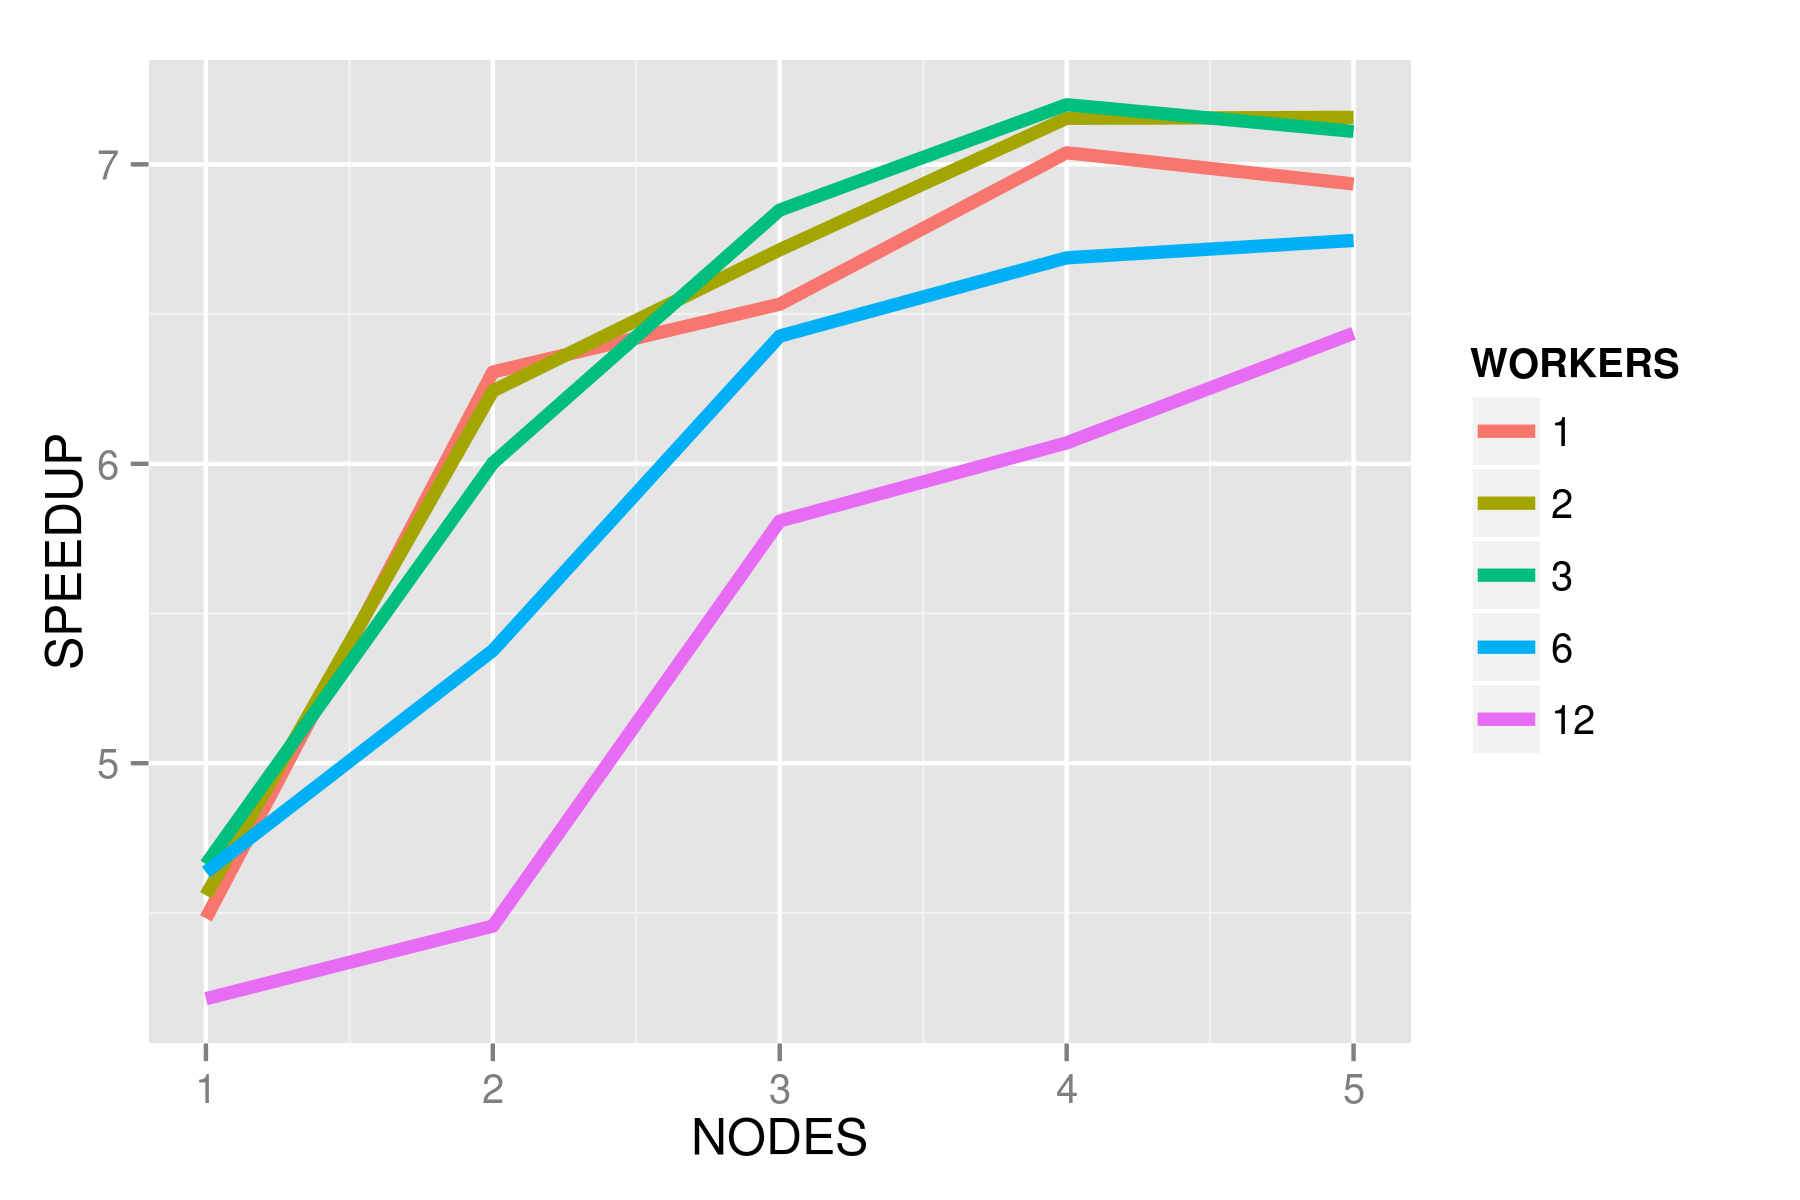
\includegraphics[width=90mm]{images/workerPerNodeSpeedup.png}
        \caption{Grep speedup with different workers per node over 20GB file}
    \end{figure}

    % efficiency graph (ref)
    % starts are less than 40% efficiency
    % drops sharply there after
    % just about 10% efficiency with 5 nodes, 60 cores

        % in graphRef we can see how well the cores are being utilized
        % in an efficiency graph
        % as expected from previous graphs, efficiency not great
        % starts under 40% efficiency with 1 node
        % end up at just about 10% efficiency with 5 nodes, or 60 cores

    \begin{figure}[H]
        \centering
        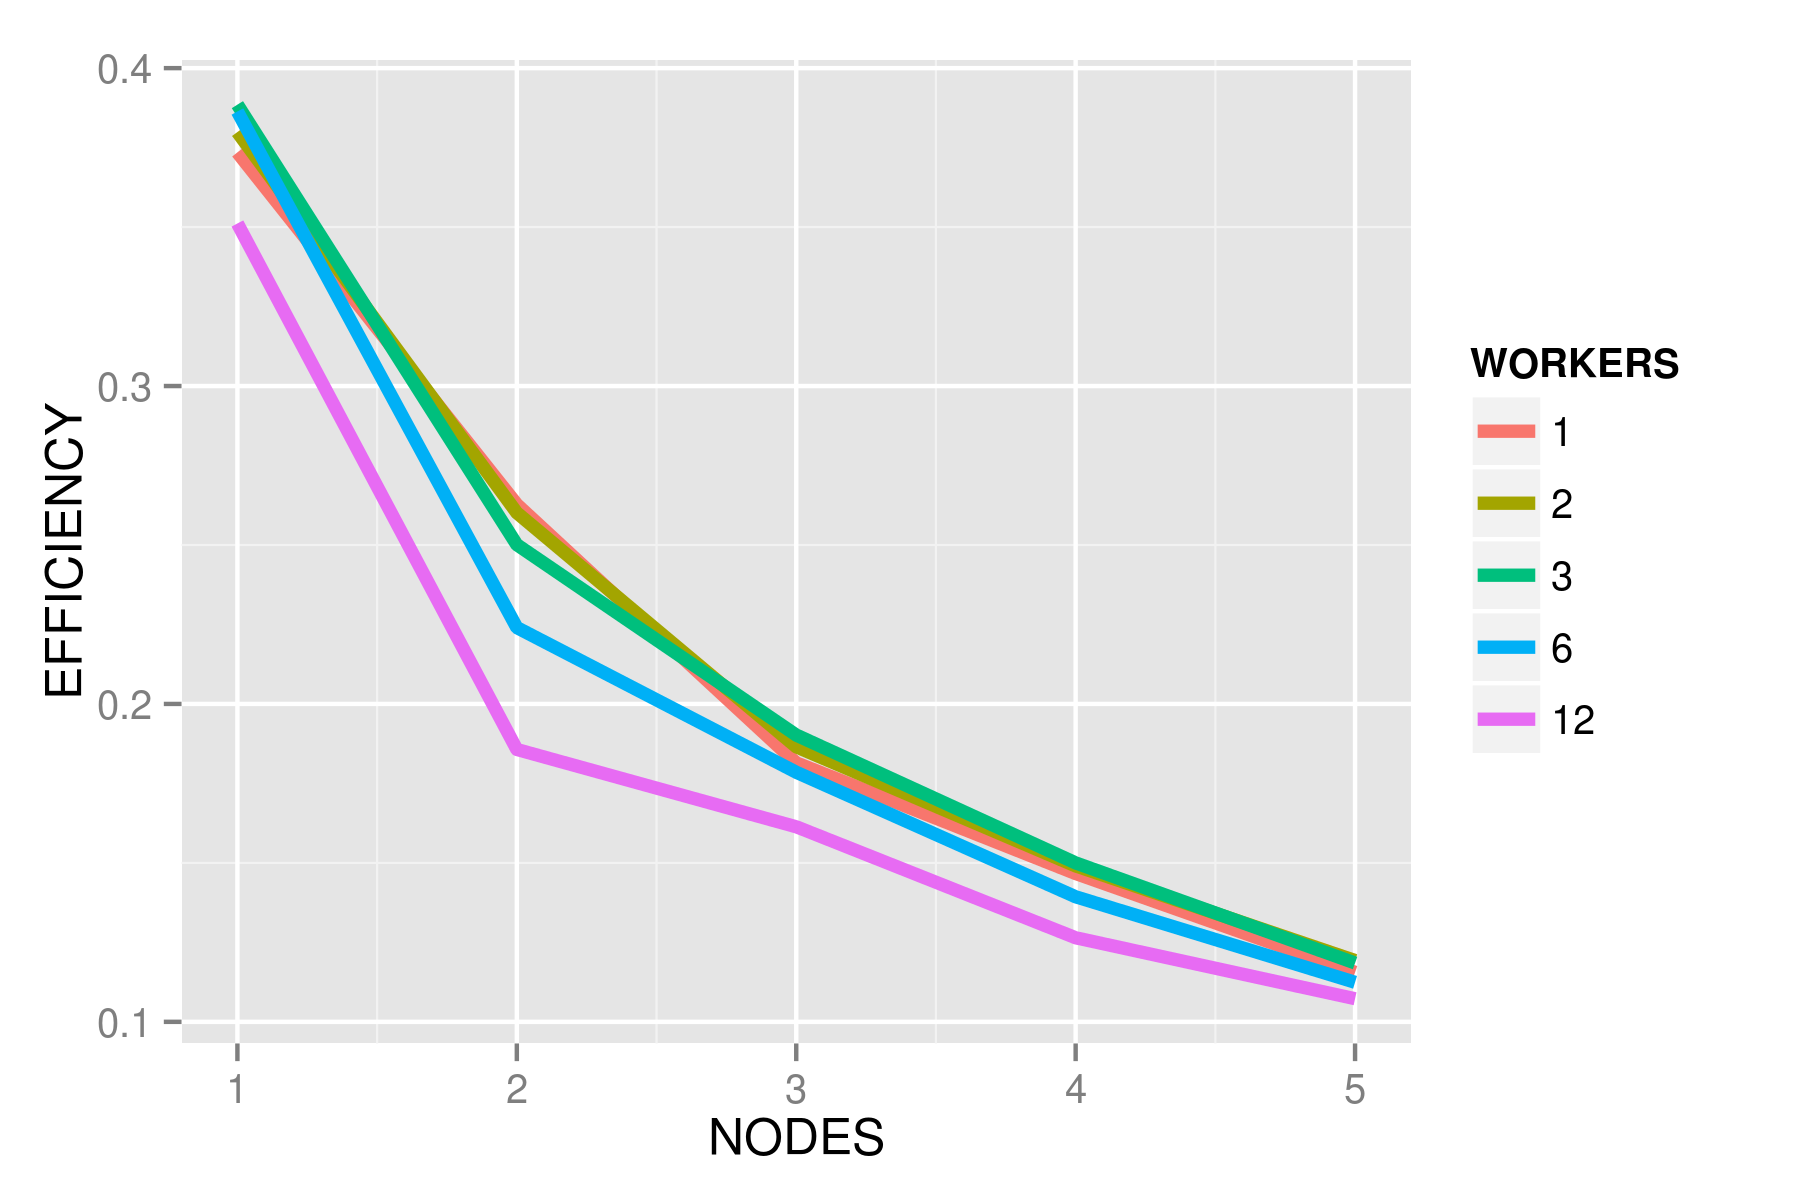
\includegraphics[width=90mm]{images/workerPerNodeEfficiency.png}
        \caption{Grep efficiency with different workers per node over 20GB file}
        \label{fig:workNodeEff}
    \end{figure}

    % karp-flatt graph (ref)
    % exception of violent changing 12 workers per node
    % stays relative constant between 0.14 and 0.12
    % suggests serial is the issue

        % finally we see this data in terms of karp-flatt metric in graphRef
        % with the exception of the 12 workers per node in pink
        % we see that the karp-flatt metric remains fairly constaint
        % values between 0.12 and 0.14
        % this constant value would suggest that the serial runtime
        % is what is preventing better scaling

    \begin{figure}[H]
        \centering
        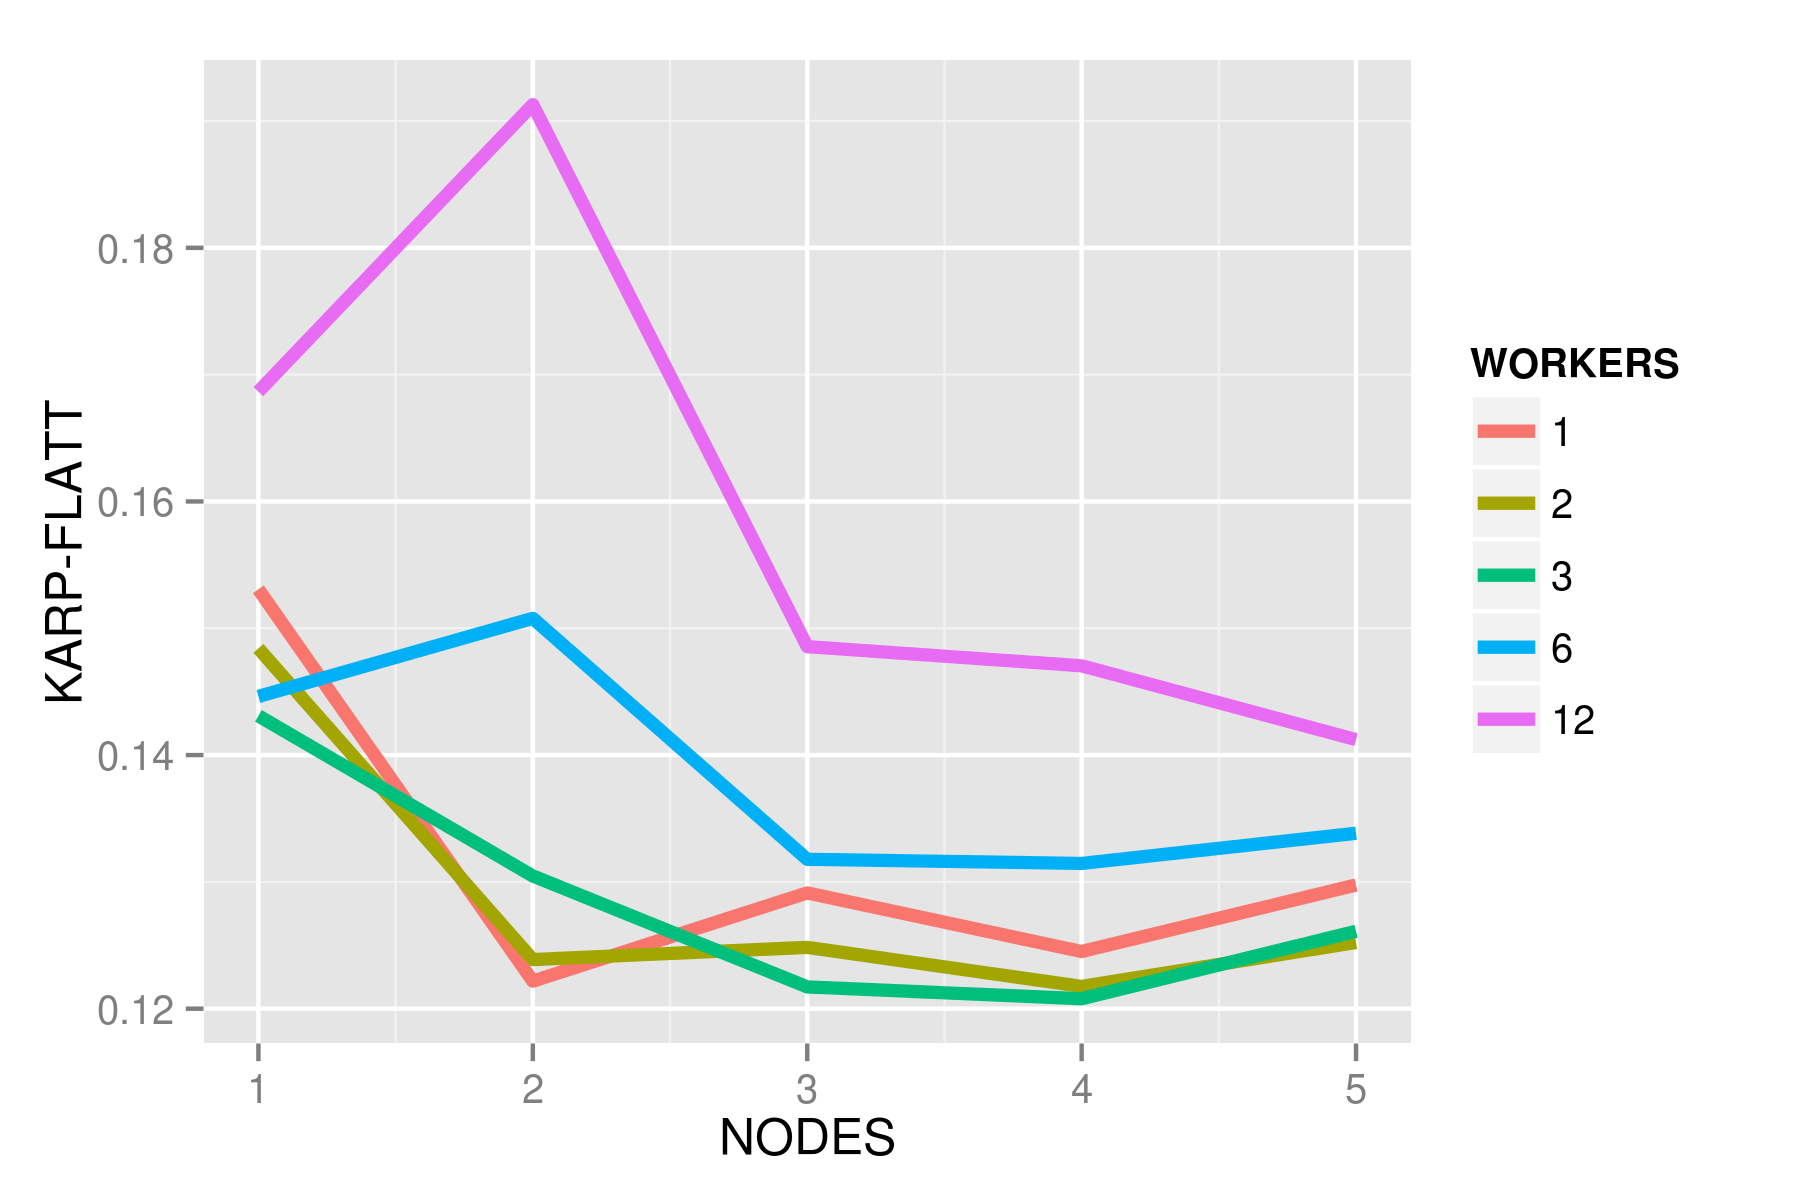
\includegraphics[width=90mm]{images/workerPerNodeKarpFlatt.png}
        \caption{Grep Karp-Flatt with different workers per node over 20GB file}
        \label{fig:workNodeKF}
    \end{figure}

% large grep test
    % serial run time (graph)
    % want to increase problem size to see better scaleup
    % clearly see no change in runtimes
    % longer compute time, PageRank, may differ

        % to see if we could see better scaling over a largest file
        % switch from 20GB to 100GB file
        % accessed file from lustre drive
        % as 100GB cannot fit in memory of one node, start with 5
        % graphRef should the runtimes over this large file
        % clearly there appears to be no change in runtimes
        % remains round 500 seconds between 5 nodes and 50
        % suspecting short compute time of grep expression
        % switch to a more computational expensive and iterative PageRank

    \begin{figure}[H]
        \centering
        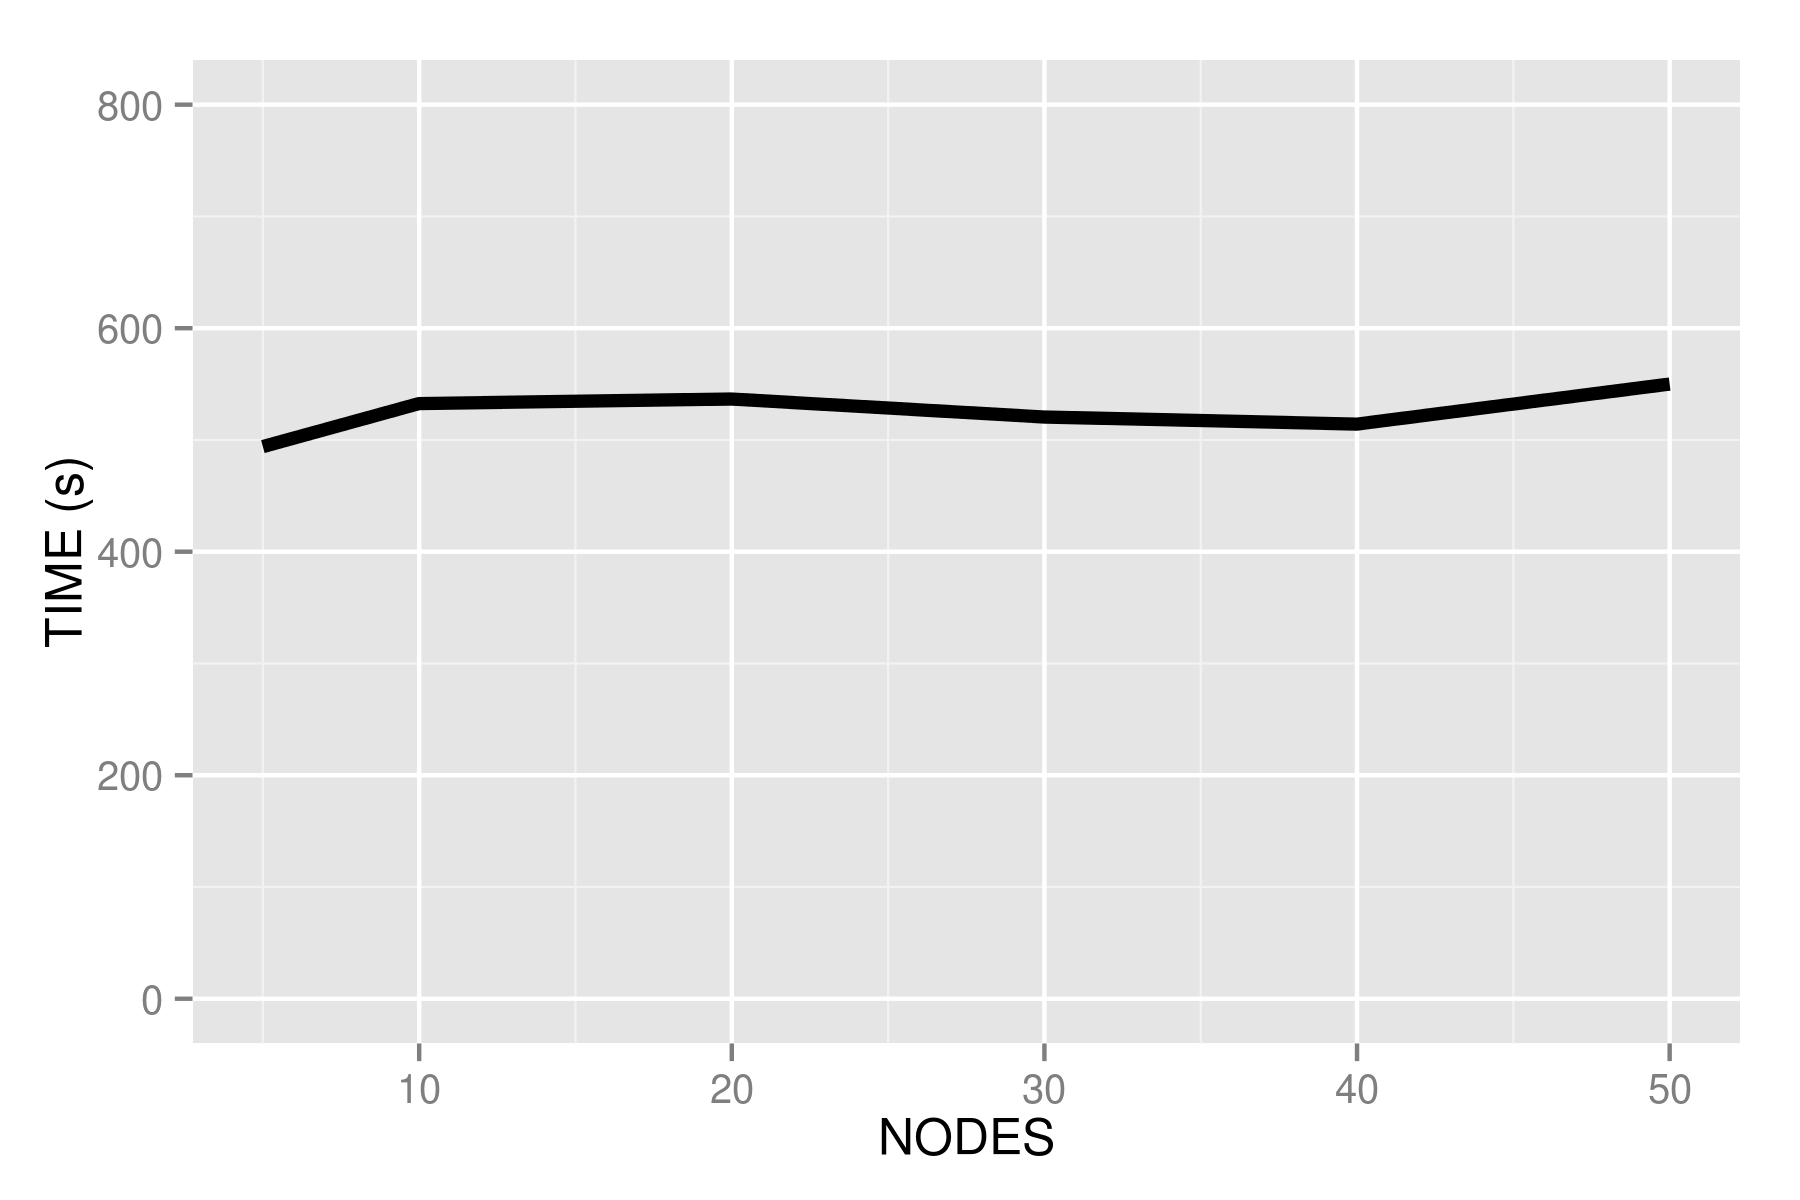
\includegraphics[width=90mm]{images/bigDataTimes.png}
        \caption{Average grep runtimes over 100GB file}
        \label{fig:bigTime}
    \end{figure}

% pagerank test 1
% pagerank test 2
% ...

\section{Discussion}
% cores grep test
    % ideal balance between speedup and efficiency
    % ideal number of workers per core 2-3
    % close enough not to matter
    % don't use 6-12

        % the results for the grep test over the 20gb file
        % gave us some insight on how well such a problem scale in spark
        % for that given task and problem size
        % 3 nodes appears to be a good balance between speedup and efficiency
        % we all saw how workers per node effects runtime
        % while 1-3 workers remains close, clear 6-12 is not ideal
        % it seems as if one my observer slightly better results
        % with 2-3 nodes over 1 node, but not by much

% large grep test
    % obvious problem with scaling
    % take away on IO
    % follow up test with delay
    % possible evidence from previous karp-flatt, serial time is factor
    % suspect file is being read in serial
    % grep can process file as load, no change in time
    % possible problem with configurations

        % in the large grep test over the 100 gb file
        % suprisingly obvserved no change in performance
        % perhaps the results of karp-flatt metric in previous test
        % gives us same insight as to why we are not seeing improvement
        % we suspect the long load times are are bigger
        % than the relatively short time needed to graph the loaded information
        % the long load times may suggest the file is not read in parallel

        % to explore this issue further, we changed our grep program
        % short pause after processing each line
        % this would negate the effects of the serial load
        % see the problem scale

% pagerank test 1
% pagerank test 2
% ...

% other problems exhibited
    % easy to install, hard to configure/profile/understand results
    % sporadic runtimes 

% workers and master communication over spark protocol

\section{Conclusion}

\bibliography{paper}
\bibliographystyle{plain}

\end{document}
